\section{'DHL Express Mobile' Application Analysis by Rafael}

The application that was analyzed in this chapter had the name 'DHL'.
The application was found on \href{https://koodous.com/apks/38ff459a46e9ea6d63a83c1eddb640626fef562cd1bcb0ab3823c4770d07d0fb}{Koodous} with the version \texttt{1.0} and package name \texttt{com.ru.dhl}, the size was \texttt{2.7 MB}.
The same package name did not exist on the Google Play Store. However, an application with the same icon was found \href{https://play.google.com/store/apps/details?id=com.dhl.exp.dhlmobile}{here}. It has the version \texttt{2.7.0}, package name \texttt{com.dhl.exp.dhlmobile} and a size of \texttt{25 MB}.

The application found on Koodous and the application found on the Google Play Store will hereinafter be referred to as 'Malicious application' and 'Original application' respectively.

\subsection{VirusTotal summary}

The malicious application was uploaded to VirusTotal to get a first impression of its capabilities.
VirusTotal indicated that the malicious application was marked by 33/63 security vendors as malicious, 
and that the original application was marked by 0/60 security vendors as malicious.

The malicious application was primarily marked as a Banker\footnote{A banker generally is an application that attempts to steal banking information in order to steal the user's money.\label{footnote-banker}}. 
If it was not marked as a banker it was either marked as a Trojan\footnote{A Trojan (or 'Trojan Horse malware') is a blanket term for malicious software that disguises itself as a harmless application\label{footnote-trojan}} or a non repeating name.
This was the full list


\begin{tabular}{ |l|l| }
    \hline
    \textbf{Vendor} & \textbf{Detection} \\
    
    \hline
        Ad-Aware    &   Trojan.GenericKD.37488882 \\
    \hline
        Alibaba     &   TrojanSpy:Android/Banker.66c12705 \\
    \hline
        Antiy-AVL   &   Trojan/Generic.ASMalwAD.5B \\
    \hline
        Arcabit     &   Trojan.Generic.D23C08F2 \\
    \hline
        Avast-Mobile    &   APK:RepSandbox [Trj] \\
    \hline
        Avira (no cloud)    &   ANDROID/Spy.Banker.YD.Gen \\
    \hline
        BitDefender     &   Trojan.GenericKD.37488882 \\
    \hline
        BitDefenderFalx     &   Android.Trojan.Banker.WS \\
    \hline
        CAT-QuickHeal   &   Android.AbereBot.Af9d \\
    \hline
        Cynet   &   Malicious (score: 99) \\
    \hline
        DrWeb   &   Android.BankBot.852.origin \\
    \hline
        Emsisoft    &   Trojan.GenericKD.37488882 (B) \\
    \hline
        eScan   &   Trojan.GenericKD.37488882 \\
    \hline
        ESET-NOD32  &   A Variant Of Android/Spy.Banker.AZU \\
    \hline
        F-Secure    &   Malware.ANDROID/Spy.Banker.YD.Gen \\
    \hline
        FireEye     &   Trojan.GenericKD.37488882 \\
    \hline
        Fortinet    &   Android/AbereBot.A!tr \\
    \hline
        GData   &   Trojan.GenericKD.37488882 \\
    \hline
        Gridinsoft  &   Trojan.U.Banker.oa \\
    \hline
        Ikarus  &   Trojan.AndroidOS.Banker \\
    \hline
        K7GW    &   Spyware ( 005817811 ) \\
    \hline
        Kaspersky   &   HEUR:Trojan-Banker.AndroidOS.AbereBot.a \\
    \hline
        Kingsoft    &   Android.Troj.tn-banker.azu.(kcloud) \\
    \hline
        Lionic  &   Trojan.AndroidOS.AbereBot.C!c \\
    \hline
        MAX     &   Malware (ai Score=100) \\
    \hline
        McAfee  &   Artemis!4778ACA48D17 \\
    \hline
        McAfee-GW-Edition   &   Artemis!Trojan \\
    \hline
        Microsoft   &   TrojanSpy:AndroidOS/Banker.GV!MTB \\
    \hline
        Symantec    &   Trojan.Gen.MBT \\
    \hline
        Symantec Mobile Insight     &   AppRisk:Generisk \\
    \hline
        Tencent     &   A.privacy.AnubisTrojanBanking \\
    \hline
        Trustlook   &   Android.Malware.Trojan \\
    \hline
        ZoneAlarm by Check Point    &   HEUR:Trojan-Banker.AndroidOS.AbereBot.a \\
    \hline
\end{tabular}
\subsubsection{Permission requests}

This chapter will describe the permissions requested by the malicious and original application.

\subsubsubsection{Malicious application}
The malicious application requested the following permissions:

\texttt{android.permission.ACCESS\_NETWORK\_STATE}
\newline \texttt{android.permission.ACCESS\_WIFI\_STATE}
\newline \texttt{android.permission.CALL\_PHONE}
\newline \texttt{android.permission.CHANGE\_WIFI\_STATE}
\newline \texttt{android.permission.FOREGROUND\_SERVICE}
\newline \texttt{android.permission.INTERNET}
\newline \texttt{android.permission.MODIFY\_AUDIO\_SETTINGS}
\newline \texttt{android.permission.READ\_CALL\_LOG}
\newline \texttt{android.permission.READ\_CONTACTS}
\newline \texttt{android.permission.READ\_PHONE\_STATE}
\newline \texttt{android.permission.READ\_PRIVILEGED\_PHONE\_STATE}
\newline \texttt{android.permission.READ\_SMS}
\newline \texttt{android.permission.RECEIVE\_BOOT\_COMPLETED}
\newline \texttt{android.permission.RECEIVE\_SMS}
\newline \texttt{android.permission.REQUEST\_DELETE\_PACKAGES}
\newline \texttt{android.permission.REQUEST\_IGNORE\_BATTERY\_OPTIMIZATIONS}
\newline \texttt{android.permission.SEND\_SMS}
\newline \texttt{android.permission.SHUTDOWN}
\newline \texttt{android.permission.UPDATE\_DEVICE\_STATS}
\newline \texttt{android.permission.WAKE\_LOCK}
\newline \texttt{android.permission.WRITE\_CALL\_LOG}
\newline \texttt{android.permission.WRITE\_CONTACTS}

There were definitely were some interesting permissions requested, for example the DHL application would under no circumstances need to read the contacts.

\newpage
\subsubsubsection{Original application}
The original application requested the following permissions:

\texttt{android.permission.CALL\_PHONE}
\newline \texttt{android.permission.FLASHLIGHT}
\newline \texttt{android.permission.READ\_APP\_BADGE}
\newline \texttt{android.permission.READ\_EXTERNAL\_STORAGE}
\newline \texttt{android.permission.READ\_PHONE\_STATE}
\newline \texttt{android.permission.USE\_FINGERPRINT}
\newline \texttt{android.permission.WRITE\_EXTERNAL\_STORAGE}
\newline \texttt{com.anddoes.launcher.permission.UPDATE\_COUNT}
\newline \texttt{com.dhl.exp.dhlmobile.permission.C2D\_MESSAGE}
\newline \texttt{com.google.android.c2dm.permission.RECEIVE}
\newline \texttt{com.htc.launcher.permission.READ\_SETTINGS}
\newline \texttt{com.htc.launcher.permission.UPDATE\_SHORTCUT}
\newline \texttt{com.huawei.android.launcher.permission.CHANGE\_BADGE}
\newline \texttt{com.huawei.android.launcher.permission.READ\_SETTINGS}
\newline \texttt{com.huawei.android.launcher.permission.WRITE\_SETTINGS}
\newline \texttt{com.majeur.launcher.permission.UPDATE\_BADGE}
\newline \texttt{com.oppo.launcher.permission.READ\_SETTINGS}
\newline \texttt{com.oppo.launcher.permission.WRITE\_SETTINGS}
\newline \texttt{com.sec.android.provider.badge.permission.READ}
\newline \texttt{com.sec.android.provider.badge.permission.WRITE}
\newline \texttt{com.sonyericsson.home.permission.BROADCAST\_BADGE}
\newline \texttt{com.sonymobile.home.permission.PROVIDER\_INSERT\_BADGE}
\newline \texttt{me.everything.badger.permission.BADGE\_COUNT\_READ}
\newline \texttt{me.everything.badger.permission.BADGE\_COUNT\_WRITE}

It was quite interesting to see how little of the permissions were common between the malicious and original application.
This indicated that the malicious application was no repackaged.
\subsection{Behavior analysis}

As soon as the application was installed it would constantly give a popup telling the user to enable Chrome. 
It also would constantly open a window showing the user how to "enable Chrome". 
If the user tried to force the app to close via these settings it would not work. 
The app would constantly open and force the user to enable the app until it was either uninstalled or enabled.
 
Touching the popup would redirect the user to the Accessibility settings. 
In this menu it would be possible to enable the malicious app. 
What it enabled would not have been shown on these settings.

If the user enabled this setting the application would disappear from the main menu and silently run in the background. 
According to the phone the app would take a lot of battery life, because it would constantly give popups asking to close background applications to save battery power. 
These popups would however be instantly closed by the application.

The only way the user would be able to find this app would be in the application settings. 
Any attempts from the user to remove the app at this stage would be thwarted by the app.
This is shown on figure \ref{tim-appbehavior}

\begin{figure}[H]
    \centering
    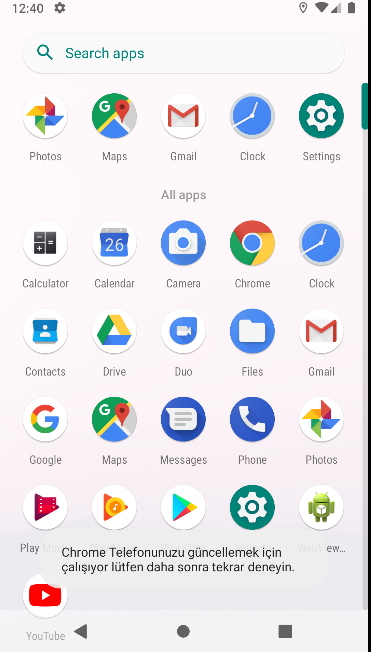
\includegraphics[width=4cm, height=15cm, keepaspectratio]{behaviorimg.png}
    \caption{app booting you from application settings}
    \label{tim-appbehavior}
\end{figure}

The message that the user would have been met with when trying to edit the application settings of the malicious chrome app translated to: 
Chrome is working to update your phone please try again later.

According to the translater this was Turkish hinting that this app might have been made by a Turkish developer.
If the application has reached this stage it would be impossible to remove it from a normal phone.



\newpage
\subsection{Network analysis}

<what does the network traffic look like>

\subsubsection{HTTP proxy analysis}

<what did the proxy reveal about the network traffic>

\subsubsection{Wireshark analysis}

<what did WireShark reveal about the network traffic>

\subsubsection{Reconnaissance [optional]}

<what was found using shodan.io>

\newpage
\subsection{Code analysis}

<interesting stuff found in code>

\newpage
\subsection{Process analysis}

<interesting stuff found in the process and memory, etc.>

\newpage
\subsection{Countermeasures and detection}

\subsubsection{Preventive measures}


<Measures to prevent installing this application>

\subsubsection{Detective measures}

<Measures to detect if this application is installed>

\subsubsection{Reactive measures}

<What to do if it is installed>

\subsubsection{YARA rule set}

<A YARA rule set created based on your findings>
